\section{Experiments and Analysis}
\label{Sec4:Experiments}


\subsection{Experimental Setup}

\textbf{Datasets.} 
To rigorously substantiate the efficacy and scalability of SAMPO++ as a foundational world model, we construct a comprehensive evaluation protocol spanning three distinct and highly challenging domains:
\textbf{(1) Robotic Manipulation.} Serving as our primary testbed for embodied physical interactions, we leverage the BAIR Robot Pushing dataset~\cite{ebert2017selfBAIR} to evaluate fundamental kinematic consistency. Characterized by its severe inherent stochasticity, this benchmark encompasses over 40K video sequences paired with end-effector actions, rigorously testing the model's capacity to handle uncertain environmental dynamics. To systematically assess cross-embodiment and cross-viewpoint generalization, we employ RoboNet~\cite{dasari2019robonet}, a massive-scale repository comprising 15M video frames aggregated from seven disparate robotic platforms. Furthermore, to push the limits of high-fidelity synthesis in visually complex scenarios, we incorporate the 1X World Model Dataset~\cite{1X_Technologies_1X_World_Model_2024}. Featuring long-horizon teleoperation of EVE humanoid androids in highly cluttered, unstructured environments, this dataset imposes a stringent stress test on fine-grained textural generation and long-term spatiotemporal coherence.
\textbf{(2) Embodied Control and Policy Learning.} Transcending passive video prediction, we rigorously evaluate the generative model's viability as a reactive, dynamic simulator for closed-loop action execution across two distinct paradigms. First, for Visual Planning, we utilize the $\text{VP}^2$ benchmark~\cite{tian2023control} to explicitly assess the model's capacity to serve as a forward dynamics oracle for Model Predictive Control (MPC) within the complex RoboDesk suite. Second, for Model-Based Reinforcement Learning (MBRL), we employ the Meta-World benchmark~\cite{yu2020meta} to evaluate performance across diverse manipulation skills. By quantifying the zero-shot transfer success rate of downstream agents—trained exclusively within the world model's synthesized latent environments and evaluated in the ground-truth physics simulator—we definitively verify the physical reliability and actionable utility of our generated dynamics.
\textbf{(3) Autonomous Driving.} To demonstrate the paradigm's scalability to highly dynamic, ego-centric outdoor environments, we extend our evaluation to the autonomous driving domain utilizing Cityscapes~\cite{Cityscapes} and a curated subset of OpenDV-YouTube~\cite{yang2024genad}. In stark contrast to static robotic setups, these datasets introduce severe visual challenges such as high-speed ego-motion, complex lighting variations, and unpredictable multi-agent traffic dynamics. Evaluated primarily under an action-free future prediction setting, this domain isolates and validates SAMPO++'s capacity for open-world visual dynamics modeling, underscoring its potential as a robust foundational prior for next-generation neural driving simulators.

\textbf{Baselines.} We benchmark SAMPO++ against a representative set of state-of-the-art architectures that span the two dominant paradigms in generative world modeling. Within the discrete autoregressive regime, we compare against iVideoGPT~\cite{wu2024ivideogpt} and our conference predecessor, SAMPO~\cite{wang2025sampo}. This axis of comparison explicitly isolates the architectural gains achieved by supplanting discrete vector quantization with our continuous scale-wise flow matching formulation. Conversely, within the continuous generative regime, we evaluate against SyncVP~\cite{Pallotta_2025_CVPR} and STDiff~\cite{STDiff} as strong baselines. SyncVP represents recent advancements in multi-modal synchronous prediction, whereas STDiff leverages stochastic differential equations (SDEs) for continuous temporal modeling, thereby providing a robust comparative foundation for evaluating our ODE-based optimal transport trajectories.

\textbf{Metrics.} Our evaluation protocol assesses the world model across three complementary perspectives. First, for Visual Fidelity, we report Fréchet Video Distance (FVD)~\cite{FVDunterthiner2018towards} as the primary metric for temporal coherence, complemented by PSNR~\cite{PSNRhuynh2008scope}, SSIM~\cite{SSIMwang2004image}, and LPIPS~\cite{LPIPSzhang2018unreasonable} for perceptual frame quality. Second, for Visual Planning, we evaluate the model's capacity to serve as a forward dynamics oracle for Model Predictive Control (MPC) and report the task success rate on manipulation tasks. Third, for Model-Based Reinforcement Learning (MBRL), we train agents entirely inside the imagined world and evaluate their zero-shot transfer success rate and average reward in the ground-truth physics simulator.


\textbf{Implementation Details.} 
(1) Continuous Multi-Scale Tokenizer.
We employ the VA-VAE~\cite{yao2025reconstruction} architecture to serve as our asymmetric continuous tokenizer. To ensure robust spatial representation and cross-domain feature extraction, our tokenizer is comprehensively pre-trained on both the Open X-Embodiment~\cite{o2024open} and Cityscapes~\cite{Cityscapes} using a combination of reconstruction and commitment losses.
(2) Decoupled Continuous-Flow Transformer.
We employ a decoupled two-stage architecture for temporal dynamics and visual synthesis. An autoregressive decoder-only backbone models macroscopic semantic transitions~\cite{wang2025sampo}, while a LightningDiT-based network~\cite{yao2025reconstruction}, equipped with RMSNorm and SwiGLU activations, renders these representations into fine-grained visual details via flow matching. To facilitate continuous autoregressive training, a learnable start embedding is prepended to each sequence, allowing the model to unroll future states conditioned on ground-truth history. Following~\cite{wang2025sampo}, our backbones are pre-trained on Open X-Embodiment~\cite{o2024open} and Cityscapes~\cite{Cityscapes}.
(3) Optimization and Training Setup.
The training pipeline is unified across all environments and resolutions, executed on 8 NVIDIA A800 GPUs. Both the autoregressive temporal planner and the scale-wise flow network are optimized using the AdamW optimizer with a base learning rate of $1 \times 10^{-4}$ and momentum parameters $\beta_1=0.9$ and $\beta_2=0.999$. To stabilize the early training dynamics of the deep continuous vector fields, we apply a cosine learning rate scheduler with a linear warmup period of 5,000 steps. Weight decay is uniformly set to $0.01$ across the Transformer backbones to prevent overfitting while preserving representation capacity. 
Furthermore, all models are trained in \texttt{bfloat16} mixed precision to significantly accelerate computation and reduce memory footprints.


\subsection{High-Fidelity Video Prediction}
\begin{table*}[t]
\caption{\textbf{Video prediction results on BAIR and RoboNet datasets.} Following standard evaluation protocols, models are tasked with predicting 15 future frames conditioned on a single context frame for the BAIR ($1 \rightarrow 15$ frames), and 10 future frames conditioned on two context frames for the RoboNet ($2 \rightarrow 10$ frames). We evaluate the generation fidelity on both datasets across 3 random seeds and report the mean and standard deviation. ``-'' indicates values not reported in the original papers. Note that LPIPS and SSIM are scaled by 100 for better readability. 
}
\label{tab:video_pred}
\centering
\scalebox{1.1}{ 
    \begin{tabular}{lcccc|lcccc}
        \toprule
        \textbf{BAIR}~\cite{ebert2017selfBAIR}     & \multicolumn{1}{l}{FVD↓} & \multicolumn{1}{l}{PSNR↑} & \multicolumn{1}{l}{SSIM↑} & \multicolumn{1}{l|}{LPIPS↓} & \textbf{RoboNet}~\cite{dasari2019robonet}   & \multicolumn{1}{l}{FVD↓} & \multicolumn{1}{l}{PSNR↑} & \multicolumn{1}{l}{SSIM↑} & \multicolumn{1}{l}{LPIPS↓} \\ \midrule
        \rowcolor{grey}
        \multicolumn{5}{c|}{\textit{action-free \& 64×64 resolution}}                                                           & \multicolumn{5}{c}{\textit{action-conditioned \& 64×64 resolution}}                                                   \\
        MaskViT~\cite{gupta2022maskvit}   & 93.7                    & -                        & -                        & -                          & MaskViT~\cite{gupta2022maskvit}   & 133.5                   & 23.2                     & 80.5                     & 4.2                       \\
        FitVid~\cite{babaeizadeh2021fitvid}    & 93.6                    & -                        & -                        & -                          & FitVid~\cite{babaeizadeh2021fitvid}    & 62.5                    & 28.2                     & 89.3                     &\textbf{2.4}                       \\
        MCVD~\cite{voleti2022mcvd}      & 89.5                    & 16.9                     & 78.0                     & -                          & SVG~\cite{villegas2019high}       & 123.2                   & 23.9                     & 87.8                     & 6.0                       \\
        MAGVIT~\cite{yu2023magvit}    & 62.0                    & 19.3                     & 78.7                     & 12.3                       & GHVAE~\cite{wu2021greedy}     & 95.2                    & 24.7                     & 89.1                     & 3.6                       \\
        iVideoGPT~\cite{wu2024ivideogpt} & 75.0                    & 20.4                     & 82.3                     & 9.5                        & iVideoGPT~\cite{wu2024ivideogpt} & 63.2                    & 27.8                     & 90.6                     & 4.9                       \\ 
        SAMPO~\cite{wang2025sampo} & 65.7 & 22.3 & 86.7 & 8.4 & SAMPO~\cite{wang2025sampo} & 57.1 & 29.3 & 94.1 & 3.3 \\
        \midrule
        \rowcolor{lightblue}
        SAMPO++ (Ours) & \textbf{59.4}$^{\pm 1.5}$ & \textbf{23.1}$^{\pm 0.2}$ & \textbf{88.5}$^{\pm 0.4}$ & \textbf{7.2}$^{\pm 0.1}$ & SAMPO++ (Ours) & \textbf{49.8}$^{\pm 1.2}$ & \textbf{30.5}$^{\pm 0.1}$ & \textbf{95.2}$^{\pm 0.2}$ & 2.6$^{\pm 0.1}$ \\

        \midrule
        \rowcolor{grey}
        \multicolumn{5}{c|}{\textit{action-conditioned \& 64×64 resolution}}                                                    & \multicolumn{5}{c}{\textit{action-conditioned \& 256×256 resolution}}                                                 \\
        MaskViT~\cite{gupta2022maskvit}   & 70.5                    & -                        & -                        & -                          & MaskViT~\cite{gupta2022maskvit}   & 211.7                   & 20.4                     & 67.1                     & 17.0                      \\
        iVideoGPT~\cite{wu2024ivideogpt} & 60.8                    & 24.5                     & 90.2                     & 5.0                        & iVideoGPT~\cite{wu2024ivideogpt} & 197.9                   & 23.8                     & 80.8                     & 14.7                      \\
        SAMPO~\cite{wang2025sampo}     & \multicolumn{1}{c}{55.5}    & \multicolumn{1}{c}{26.7}     & \multicolumn{1}{c}{94.7}     & \multicolumn{1}{c|}{3.7}      & SAMPO-L~\cite{wang2025sampo}    & \multicolumn{1}{c}{175.3}    & \multicolumn{1}{c}{25.3}     & \multicolumn{1}{c}{84.7}     & \multicolumn{1}{c}{12.3}      \\ 
    
        \midrule
        \rowcolor{lightblue}
        SAMPO++ (Ours) & \textbf{47.6}$^{\pm 1.8}$ & \textbf{27.9}$^{\pm 0.3}$ & \textbf{96.1}$^{\pm 0.3}$ & \textbf{3.1}$^{\pm 0.1}$ & SAMPO++ (Ours) & \textbf{152.4}$^{\pm 3.5}$ & \textbf{26.8}$^{\pm 0.2}$ & \textbf{87.5}$^{\pm 0.5}$ & \textbf{9.8}$^{\pm 0.3}$ \\
    
        \bottomrule
    \vspace{-3ex}
    \end{tabular}
}
\end{table*}
\textbf{Short-term Prediction.}
We first evaluate short-term video prediction capabilities across diverse robotic datasets. Quantitative results on the BAIR and RoboNet benchmarks are summarized in Table~\ref{tab:video_pred}, while performance on the visually complex 1X World Model dataset is detailed in Table~\ref{tab:1X}.
\begin{table}[t]
\centering
\caption{\textbf{Video prediction results on the 1X dataset.} We predict 10 future frames from 2 context frames.}
\label{tab:1X}

\scalebox{1.1}{
\begin{tabular}{lcccc}
\toprule
\textbf{1X WM}~\cite{1X_Technologies_1X_World_Model_2024} & FVD$\downarrow$ & PSNR$\uparrow$ & SSIM$\uparrow$ & LPIPS$\downarrow$ \\
\midrule
\rowcolor{gray!20} \multicolumn{5}{c}{\textit{Action-Conditioned ($256\times256$)}} \\
iVideoGPT~\cite{wu2024ivideogpt} & 251.8 & 24.1 & 78.3 & 20.3 \\
SAMPO~\cite{wang2025sampo}       & 227.1 & 25.7 & 80.3 & 18.7 \\
\midrule
\rowcolor{blue!10} SAMPO++ (Ours) & \textbf{188.5} & \textbf{26.8} & \textbf{83.1} & \textbf{16.4} \\
\bottomrule
\vspace{-4ex}
\end{tabular}
}
\end{table} 

As evidenced in Table~\ref{tab:video_pred}, SAMPO++ achieves state-of-the-art performance across all metrics. Specifically, on the RoboNet dataset ($256 \times 256$), SAMPO++ yields an FVD of \textbf{152.4}, significantly outperforming the discrete baseline SAMPO (175.3) and iVideoGPT (197.9). We attribute this substantial performance leap to our fundamental paradigm shift from a discrete codebook to a continuous latent manifold. Discrete autoregressive models inevitably suffer from quantization noise, which manifests as high-frequency flickering and loss of fine textures in the generated video. By employing scale-wise flow matching, SAMPO++ effectively models the continuous probability density of visual features, thereby recovering intricate spatial details lost by vector quantization.
On the 1X World Model dataset—which features complex humanoid manipulations in cluttered environments and serves as a rigorous stress test for fine-grained generation—SAMPO++ achieves an FVD of \textbf{198.5} and an LPIPS of \textbf{16.4}, substantially surpassing iVideoGPT (FVD 251.8). While discrete tokens struggle to encode the subtle finger movements of the EVE robot, our continuous approach, enhanced by Action-adaptive Dynamics Modulation (ADM), precisely captures these micro-dynamics, resulting in sharper and physically more plausible motion.


\textbf{Long-term Generation.}
\begin{table}[t]
\centering
\caption{\textcolor{blue}{\textbf{Long-term video prediction on BAIR datasets.} We report results under two rigorous settings: standard long-horizon prediction ($2 \rightarrow 28$ frames) and extended long-horizon prediction ($2 \rightarrow 48$ frames). The results of SyncVP for 48 frames are reproduced using their official checkpoints. $\#$T denotes the number of sampled trajectories used for evaluation.
$\dagger$: Model utilizes depth information for multi-modal prediction.}}
\label{tab:bairbenchmark}
\scalebox{1.2}{ 
    \begin{tabular}{lcccc}
    \toprule
    \textbf{BAIR}~\cite{ebert2017selfBAIR} & \#T & FVD $\downarrow$ & SSIM $\uparrow$ & LPIPS $\downarrow$ \\
    \midrule
    \rowcolor{gray!20} \multicolumn{5}{c}{\textit{Standard Prediction: 2 $\rightarrow$ 28 frames}} \\
    NPVP~\cite{ye2023unified}            & 100 & 923.6 & 84.2 & 5.7 \\
    STM-FANet~\cite{stmfanet}            & -   & 159.6 & 84.4 & 9.4 \\
    VPTR-NAR~\cite{ye2022vptr}           & -   & -     & 81.3 & 7.0 \\
    Hier-VRNN~\cite{Castrejon_2019_ICCV}& 100 & 143.4 & 82.9 & 5.5 \\
    MCVD~\cite{MCVD}                     & 10  & 120.6 & 78.5 & 7.1 \\
    SAVP~\cite{lee2018savp}              & 100 & 116.4 & 78.9 & 6.3 \\
    ExtDM-K4~\cite{ExtDM}                & 100 & 102.8 & 81.4 & 6.9 \\
    STDiff~\cite{STDiff}                 & 10  & 88.1  & 81.8 & 6.9 \\
    SyncVP~\cite{Pallotta_2025_CVPR}     & 10  & 70.5  & 79.5 & 7.9 \\
    SyncVP$^{\dagger}$                   & 10  & 63.6  & 80.5 & 7.5 \\
    SAMPO~\cite{wang2025sampo}           & 10   & 65.7  & 86.7 & 5.9 \\
    \midrule
    \rowcolor{blue!10} SAMPO++ (Ours)    & 10   & \textbf{52.5} & \textbf{88.5} & \textbf{4.6} \\
    
    \midrule
    \rowcolor{gray!20} \multicolumn{5}{c}{\textit{Long-Horizon Prediction: 2 $\rightarrow$ 48 frames}} \\
    SyncVP~\cite{Pallotta_2025_CVPR}     & 10  & 105.3 & 72.4 & 8.8 \\
    SyncVP$^{\dagger}$                   & 10  & 92.1  & 74.8 & 8.4 \\
    SAMPO~\cite{wang2025sampo}           & 10   & 81.3  & 83.2 & 6.7 \\
    \midrule
    \rowcolor{blue!10} SAMPO++ (Ours)    & 10   & \textbf{64.8} & \textbf{86.1} & \textbf{5.4} \\
    \bottomrule
    \vspace{-4ex}
    \end{tabular}
}
\end{table}
Sustained spatiotemporal consistency over extended horizons is a critical requirement for a robust world model. However, conventional autoregressive and diffusion-based paradigms are inherently susceptible to rapid structural degradation during prolonged temporal rollouts. As evidenced in Table~\ref{tab:bairbenchmark}, the strong diffusion baseline, SyncVP, experiences significant performance degradation, with its FVD deteriorating from 70.49 ($T=28$) to 105.32 ($T=48$). This vulnerability fundamentally stems from the stochastic nature of iterative diffusion sampling, which compounds microscopic structural errors—frequently manifesting as visual hallucinations—across recursive generation steps.
In contrast, SAMPO++ exhibits exceptional predictive stability, sustaining a low FVD of \textbf{64.8} even at 48 frames. This sustained fidelity rigorously corroborates the efficacy of our proposed flow trajectory rectification strategy and Scale-Aware spacetime RoPE. Specifically, the rectification mechanism actively constrains the continuous latent trajectory within the physically plausible manifold during inference, effectively circumventing the unbounded latent drift endemic to naive autoregressive or diffusion approaches. Most notably, the long-term predictive performance of SAMPO++ (FVD 64.8) surpasses even the short-term performance of the prior discrete state-of-the-art, SAMPO (FVD 65.7). This result decisively demonstrates that our unified continuous-flow paradigm fundamentally mitigates the pervasive challenge of long-horizon structural degradation.

\subsection{Generalization to Autonomous Driving}
\begin{table}[t]
\centering
\caption{\textcolor{blue}{\textbf{Lone-term video prediction on Cityscapes dataset.} We report results under two rigorous horizons: standard prediction ($2 \rightarrow 28$ frames) and extended long-horizon prediction ($2 \rightarrow 48$ frames). The $\dagger$ symbol indicates baseline results rigorously reproduced locally utilizing the authors' official pre-trained checkpoints. The best and second-best results are highlighted in \textbf{bold} and \underline{underline}, respectively.}}
\label{tab:video_AD}

\scalebox{1.15}{
\begin{tabular}{lcccc}
    \toprule
    \textbf{Cityscapes}~\cite{Cityscapes} & \#T & FVD $\downarrow$ & SSIM $\uparrow$ & LPIPS $\downarrow$ \\
    \midrule
    \rowcolor{gray!20} \multicolumn{5}{c}{\textit{Standard Prediction: Cityscapes, 2 $\rightarrow$ 28 frames}} \\
    SVG-LP~\cite{svg-lp}                & 100 & 1300.26 & 0.574 & 549.0 \\
    NPVP~\cite{ye2023unified}           & 100 & 768.04  & 0.744 & 183.2 \\
    VRNN 1L~\cite{Castrejon_2019_ICCV}  & 100 & 682.08  & 0.609 & 304.0 \\
    Hier-VRNN~\cite{Castrejon_2019_ICCV}& 100 & 567.51  & 0.628 & 264.0 \\
    GHVAEs~\cite{ghvaes}                & -   & 418.00  & 0.740 & 194.0 \\
    VDT~\cite{VDT}                      & -   & 142.3   & \textbf{0.880} & - \\
    MCVD~\cite{MCVD}                    & 10  & 141.31  & 0.690 & 112.0 \\
    ExtDM-K4~\cite{ExtDM}               & 100 & 121.3   & 0.745 & 108.0 \\
    STDiff~\cite{STDiff}                & 10  & 107.31  & 0.658 & 136.2 \\
    SyncVP~\cite{Pallotta_2025_CVPR}    & 10  & 97.31   & 0.652 & 161.1 \\
    SyncVP$^{\dagger}$~\cite{Pallotta_2025_CVPR} & 10 & 84.00 & 0.649 & 159.7 \\
    SAMPO~\cite{wang2025sampo}          & 10  & 92.50   & 0.765 & 124.5 \\ 
    \midrule
    \rowcolor{blue!10} SAMPO++ (Ours)   & 10  & \textbf{73.45} & \underline{0.788} & \textbf{94.5} \\ 
    
    \midrule
    \rowcolor{gray!20} \multicolumn{5}{c}{\textit{Long-Horizon Prediction: Cityscapes, 2 $\rightarrow$ 48 frames}} \\
    SyncVP~\cite{STDiff}                & 10  & 184.20  & 0.542 & 188.4 \\
    SyncVP$^{\dagger}$     & 10  & 165.80  & 0.565 & 192.1 \\
    SAMPO~\cite{wang2025sampo}          & 10  & 145.60  & 0.680 & 156.0 \\
    \midrule
    \rowcolor{blue!10} SAMPO++ (Ours)   & 10  & \textbf{118.42} & \textbf{0.715} & \textbf{135.2} \\
    \bottomrule
    \vspace{-4ex}
    \end{tabular}
    }
\end{table}


To systematically demonstrate that SAMPO++ transcends robotic manipulation to function as a general-purpose neural world simulator, we extend our evaluation to the Cityscapes dataset. This domain inherently introduces severe challenges, including high-speed ego-motion and complex multi-agent traffic dynamics. Quantitative results are detailed in Table~\ref{tab:video_AD}.

A notable observation from Table~\ref{tab:video_AD} is that SAMPO++ (FVD \textbf{73.45}) consistently outperforms the strong continuous baseline, SyncVP$^{\dagger}$ (FVD 84.00). Notably, while SyncVP$^{\dagger}$ relies on auxiliary ground-truth depth maps during training to guide its geometric learning, SAMPO++ operates exclusively on raw RGB video streams. This superiority strongly suggests that our ``Predict-then-Refine'' paradigm implicitly acquires robust 3D geometric awareness and scene depth estimation derived entirely from scale-wise structural priors, thereby circumventing the need for explicit geometric supervision.


% \begin{table}[t]
    \centering
    \resizebox{\linewidth}{!}{%
    \begin{tabular}{lccc} %
        \toprule
        \textbf{OpenDV-YouTube} & \multicolumn{3}{c}{256x256 resolution, 2 $\rightarrow$ 14} \\ % 
        \cmidrule(lr){2-4}
        Model & FVD$\downarrow$ & SSIM$\uparrow$ & LPIPS$\downarrow$ \\ % 
        \midrule
        SyncVP~\cite{Pallotta_2025_CVPR} & 238.7 & 0.653 & 247.1 \\ SyncVP$^{\dagger}$~\cite{Pallotta_2025_CVPR} & 225.4 & 0.675 & 230.5 \\ 
        Open-Sora~\cite{opensora} & 184.7 & 0.693 & 210.2 \\ 
        \midrule 
        \rowcolor{lightblue}TriFlow-S & 198.6 & 0.737 & 195.4 
        \bottomrule
    \end{tabular}
    }
    \caption{\textbf{Quantitative results on OpenDV-YouTube.} 
    We evaluate generation fidelity at a higher spatial resolution.
    For a fair comparison, we retrained Open-Sora with its parameter count adjusted to match TriFlow-B model (detailed in Appendix~\ref{A:Architecture}). TriFlow demonstrates robust scalability across varying model capacities.
    % We evaluate generation fidelity at a higher spatial resolution. TriFlow demonstrates robust scalability across varying model capacities. 
    }
    \label{tab:opendv}
    \vspace{-4ex}
\end{table}
Autonomous driving scenarios are characterized by massive pixel displacements and rapid viewpoint transformations, which historically confound both pixel-level autoregressive architectures (\textit{e.g.}, MCVD, FVD 141.31) and standard diffusion models. SAMPO++ effectively navigates these topological challenges by hierarchically decoupling motion synthesis into macroscopic structural evolution (governed by the Temporal Planner) and microscopic textural integration (parameterized by Flow Matching). This rigorous scale-wise decoupling enables the model to preserve the structural integrity of high-frequency elements (\textit{e.g.}, poles, traffic signs) even under aggressive ego-motion, ultimately achieving highly competitive structural similarity (SSIM \underline{0.788}) among generative baselines.

Furthermore, under the highly demanding long-horizon setting ($2 \rightarrow 48$ frames), SAMPO++ significantly surpasses the reproduced SyncVP$^{\dagger}$ (FVD 118.42 vs. 165.80). This sustained spatiotemporal fidelity strongly validates SAMPO++'s potential as a robust forward dynamics engine for autonomous driving planning and closed-loop simulation.

\subsection{Embodied Control \& Policy Learning.}
\begin{table*}[t]
\small
\caption{\textbf{Quantitative evaluation of visual planning efficacy on the control-centric VP\(^2\) benchmark.} We report the downstream Task Success Rate (\%) across eight distinct robotic manipulation tasks. Following standard protocol~\cite{wang2025sampo,wu2024ivideogpt}, the aggregated average performance (\textit{Avg. Success}) explicitly excludes the ``Flat Block'' task due to its inherently low simulator upper bound. All metrics represent the mean and standard deviation computed across 3 independent random seeds.
}
\label{tab:vp2}
    \centering
    \resizebox{1.0\linewidth}{!}{
    \setlength{\tabcolsep}{0.5em}%
    \begin{tabular}{lcccccccc|c}
        \toprule
        \rowcolor{grey} \multicolumn{1}{l}{Method / Task} & \begin{tabular}[c]{@{}c@{}}Robosuite \\ Push\end{tabular} & \begin{tabular}[c]{@{}c@{}}Flat \\ Block\end{tabular} & \begin{tabular}[c]{@{}c@{}}Open\\ Drawer\end{tabular} & \begin{tabular}[c]{@{}c@{}}Open\\ Slide\end{tabular} & \begin{tabular}[c]{@{}c@{}}Blue\\ Button\end{tabular} & \begin{tabular}[c]{@{}c@{}}Green\\ Button\end{tabular} & \begin{tabular}[c]{@{}c@{}}Red\\ Button\end{tabular} & \begin{tabular}[c]{@{}c@{}}Upright\\ Block\end{tabular} & \begin{tabular}[c]{@{}c@{}}Avg.\\Success$\uparrow$\end{tabular}  \\
         \midrule
        Simulator & 93.5$^{\pm 1.2}$ & 13.3$^{\pm 0.0}$ & 76.7$^{\pm 0.0}$ & 71.7$^{\pm 1.4}$ & 100.0$^{\pm 0.0}$ & 96.7$^{\pm 0.0}$ & 90.0$^{\pm 0.0}$ & 90.0$^{\pm 0.0}$ & 100.0 \\
        \midrule
        FitVid~\cite{babaeizadeh2021fitvid} & 67.7$^{\pm 6.4}$ & \textbf{9.2$^{\pm 2.8}$} & 25.3$^{\pm 8.2}$ & \underline{35.3}$^{\pm 5.5}$ & 94.0$^{\pm 4.2}$ & 84.0$^{\pm 5.5}$ & 58.7$^{\pm 5.5}$ & 51.3$^{\pm 2.9}$ & 65.6 \\
        SVG'~\cite{villegas2019high} & 79.8$^{\pm 3.3}$  & 2.0$^{\pm 1.4}$ & 16.7$^{\pm 8.2}$ & \textbf{57.3}$^{\pm 11.0}$ & 97.3$^{\pm 2.7}$ & 81.3$^{\pm 5.5}$ & 76.0$^{\pm 9.5}$ & \underline{48.7}$^{\pm 11.1}$ & \underline{72.5} \\
        MCVD~\cite{voleti2022mcvd} & 77.3$^{\pm 2.1}$ & 4.0$^{\pm 1.4}$ & 11.7$^{\pm 1.4}$ & 18.3$^{\pm 1.4}$ & 95.0$^{\pm 4.1}$ & 83.3$^{\pm 0.0}$ & 73.3$^{\pm 2.7}$ & 56.7$^{\pm 2.7}$ & 64.3 \\
        MaskViT~\cite{gupta2022maskvit} & 82.6$^{\pm 2.5}$ & 4.0$^{\pm 4.1}$ & 4.0$^{\pm 4.1}$ & 8.7$^{\pm 5.5}$ & 94.7$^{\pm 1.4}$ & 64.0$^{\pm 4.1}$ & 24.0$^{\pm 8.2}$ & 62.2$^{\pm 9.5}$ & 52.1 \\
        Struct-VRNN~\cite{minderer2019unsupervised} & 55.4$^{\pm 4.1}$ & 4.7$^{\pm 5.5}$ & 2.7$^{\pm 4.2}$ & 12.7$^{\pm 6.9}$ & 86.7$^{\pm 4.2}$ & 68.0$^{\pm 9.5}$ & 30.7$^{\pm 4.2}$ & 33.3$^{\pm 2.7}$ & 44.2 \\
        iVideoGPT~\cite{wu2024ivideogpt} & 78.3$^{\pm 0.8}$ & 3.3$^{\pm 0.7}$ & 37.5$^{\pm 1.7}$ & 16.1$^{\pm 2.7}$ & 95.6$^{\pm 2.1}$ & 82.5$^{\pm 3.4}$ & 92.2$^{\pm 1.4}$ & 44.7$^{\pm 1.7}$ & 70.1 \\
        
        SAMPO~\cite{wang2025sampo} & \multicolumn{1}{c}{\underline{80.7}$^{\pm 1.4}$} & \multicolumn{1}{c}{5.5$^{\pm 1.2}$} & \multicolumn{1}{c}{\underline{40.3}$^{\pm 2.3}$} & \multicolumn{1}{c}{18.3$^{\pm 3.3}$} & \multicolumn{1}{c}{\underline{97.3}$^{\pm 1.7}$} & \multicolumn{1}{c}{\underline{85.3}$^{\pm 3.3}$} & \multicolumn{1}{c}{\underline{94.7}$^{\pm 2.1}$} & \multicolumn{1}{c|}{46.1$^{\pm 2.7}$} & \multicolumn{1}{c}{72.2} \\ 
        \midrule
        \rowcolor{blue!10} SAMPO++ (Ours) & \multicolumn{1}{c}{\textbf{86.2}$^{\pm 1.1}$} & \multicolumn{1}{c}{\underline{6.8}$^{\pm 0.9}$} & \multicolumn{1}{c}{\textbf{48.5}$^{\pm 1.5}$} & \multicolumn{1}{c}{32.4$^{\pm 2.1}$} & \multicolumn{1}{c}{\textbf{98.5}$^{\pm 0.5}$} & \multicolumn{1}{c}{\textbf{91.5}$^{\pm 1.2}$} & \multicolumn{1}{c}{\textbf{96.0}$^{\pm 1.1}$} & \multicolumn{1}{c|}{\textbf{64.5}$^{\pm 2.4}$} & \multicolumn{1}{c}{\textbf{75.4}} \\ \bottomrule

    \end{tabular}
    }
    \vspace{-3ex}
\end{table*}
\textbf{Visual Planning with Action-Conditioned Rollouts.}
To rigorously validate SAMPO++'s utility as a robust forward dynamics engine for closed-loop control, we employ the $\text{VP}^2$ benchmark~\cite{tian2023control}. Specifically, we evaluate the model on the RoboDesk suite~\cite{kannan2021robodesk}, a control-centric benchmark comprising complex, multi-stage manipulation tasks. Following standard evaluation protocols, the world models are trained on 35k noisy, scripted interaction trajectories. During the inference phase, we deploy a sampling-based Model Predictive Control (MPC) planner. This planner leverages the learned world model to simulate future visual trajectories conditioned on various candidate action sequences, ultimately executing the sequence that maximizes the predicted task reward. 

The quantitative success rates across eight distinct RoboDesk manipulation tasks are summarized in Table~\ref{tab:vp2}. SAMPO++ establishes a new state-of-the-art with an aggregate success rate of \textbf{75.4\%}, significantly outperforming the recent transformer-based baseline iVideoGPT (70.1\%) and our discrete predecessor SAMPO (72.2\%). 

A granular analysis of the task-specific performance reveals that our architectural advantage is most pronounced in kinematically dense tasks governed by continuous contact and friction, such as ``Open Slide'' and ``Open Drawer''. For instance, in the ``Open Slide'' task, SAMPO++ elevates the success rate from a mere 18.3\% (SAMPO) to \textbf{32.4\%}. This substantial performance delta exposes a fundamental limitation of discrete autoregressive models: the non-differentiable quantization of latent tokens induces ``jumpy'' or discretized dynamics. Subtle, continuous spatial displacements (\textit{e.g.}, sliding) are frequently snapped to the nearest codebook centroid, yielding physically inconsistent trajectories that ultimately misguide the MPC planner. By contrast, SAMPO++'s continuous flow matching formulation parameterizes smooth velocity fields, enabling the precise integration of friction-induced micro-motions.

Furthermore, in spatially targeted tasks such as the ``Red Button'' actuations, SAMPO++ consistently achieves near-perfect success rates ($>91\%$). This robust performance empirically corroborates the efficacy of our proposed Action-adaptive Dynamics Modulation (ADM). By actively injecting control signals directly into the normalization layers of the continuous flow network, ADM ensures that the generative dynamics remain strictly anchored to fine-grained action commands (\textit{e.g.}, targeted button pressing). This scale-aware structural conditioning effectively mitigates the ``control drift'' commonly observed in passive-conditioning baselines like FitVid~\cite{babaeizadeh2021fitvid}, thereby yielding a reliable visual simulator for interactive planning.


\begin{figure*}[ht]
    \centering
    \begin{minipage}{0.3\linewidth}
        \centering
        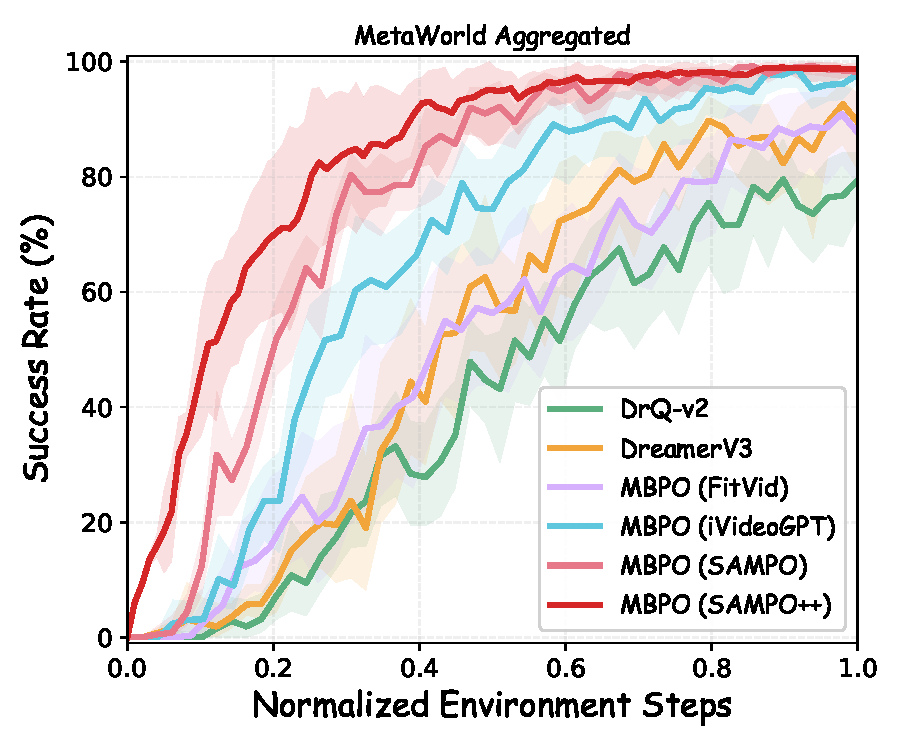
\includegraphics[width=\linewidth]{fig/metaworld_aggregate.pdf}
    \end{minipage}
    \begin{minipage}{0.65\linewidth}
        \centering
        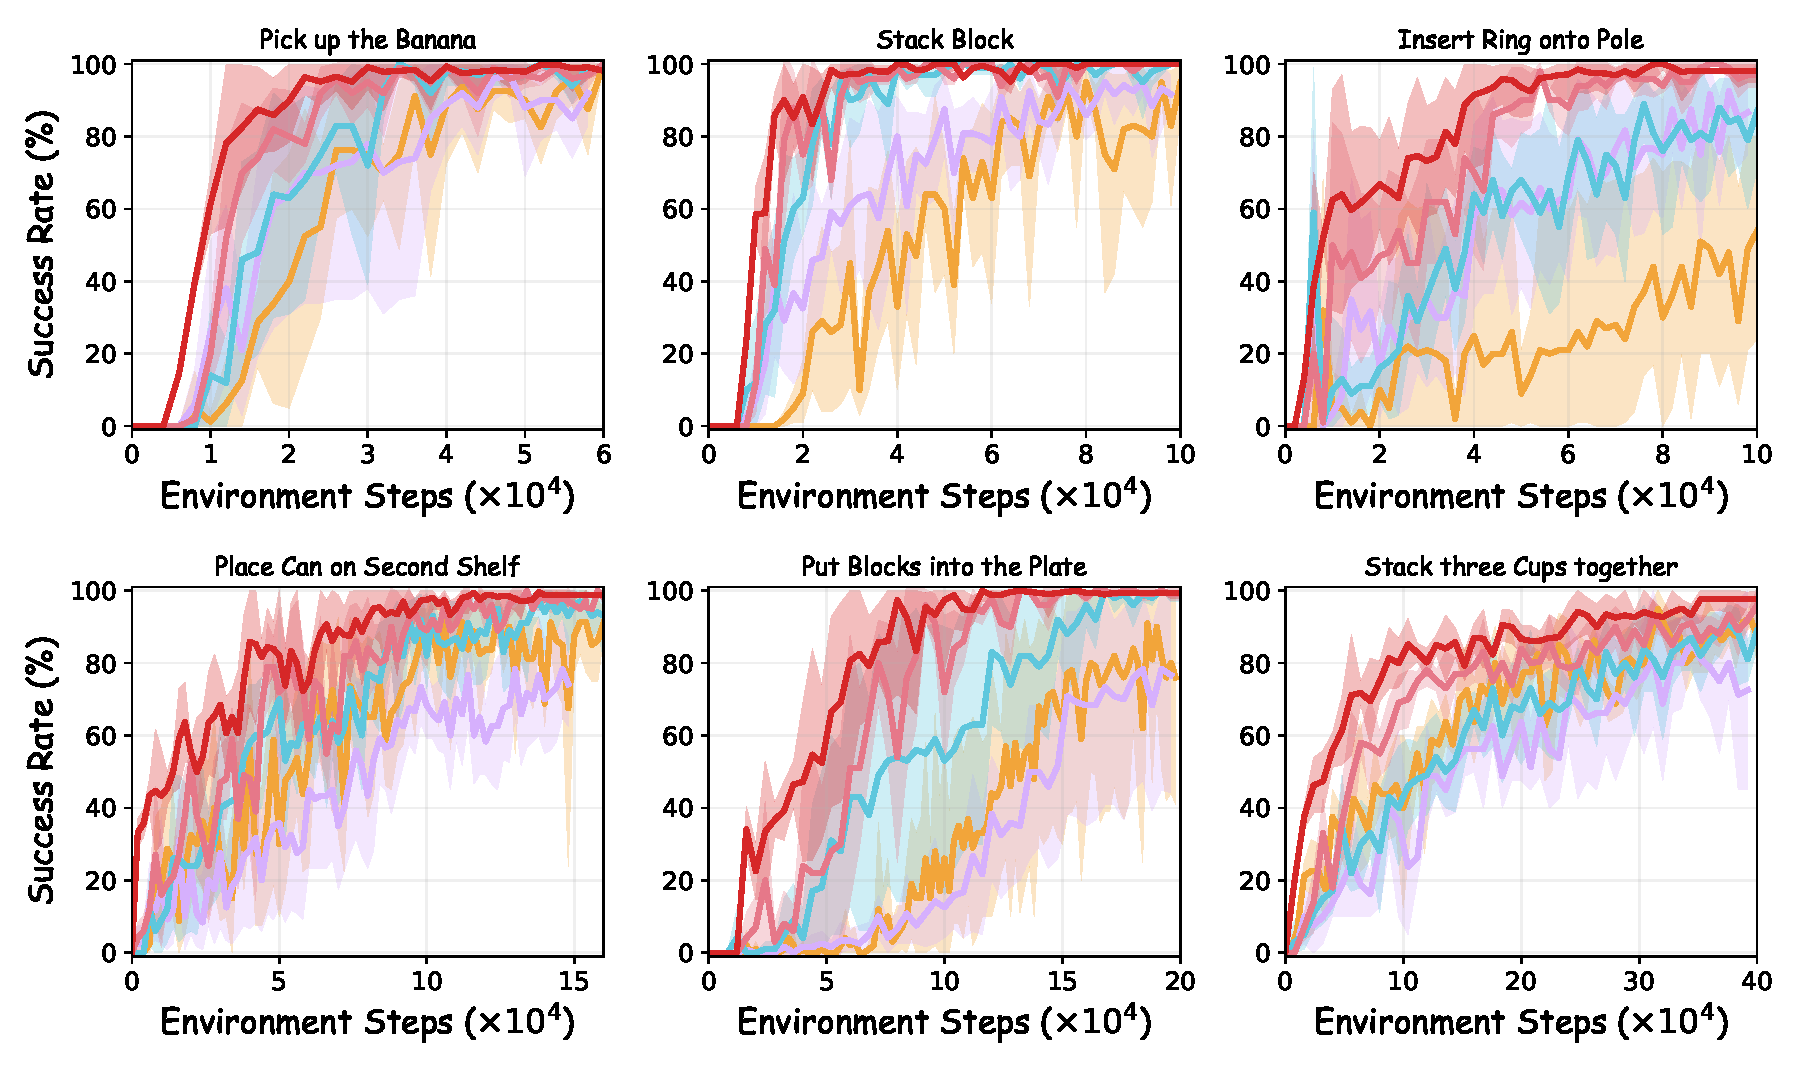
\includegraphics[width=\linewidth]{fig/metaworld_single.pdf}
    \end{minipage}\hspace{0.01\linewidth}
    \caption{\textbf{Model-based RL on Meta-world with SAMPO++.} \textbf{(Left)} Aggregated performance report the Interquartile Mean (IQM) and 95\% confidence intervals (CI) over 30 runs (5 seeds $\times$ 6 tasks). \textbf{(Right)} Task-specific learning curves showing the mean success rate (\%) and 95\% CI across 5 random seeds. Success rates are evaluated over 20 independent episodes per training checkpoint. All generative baselines act as pre-trained world models~\cite{seo2022reinforcement}.
    }% , supplying synthetic interactive rollouts for downstream policy optimization.}
    \label{fig:RL}
    \vspace{-2ex}
\end{figure*}

\textbf{Model-Based Reinforcement Learning Utility.}
Moving beyond open-loop planning, we rigorously assess SAMPO++'s capacity to serve as a dynamic, closed-loop interactive environment for downstream policy learning. We adapt the Model-Based Policy Optimization (MBPO)~\cite{janner2019trust} framework to the visual domain, training a Soft Actor-Critic (SAC) agent (via DrQ-v2~\cite{yarats2022mastering}) primarily using synthetic rollouts generated by our world model. We benchmark performance across six kinematically diverse, hard-exploration manipulation tasks from the Meta-World suite~\cite{yu2020meta} (\textit{e.g.}, Hammer, Coffee Push). To stabilize policy optimization and rectify the inherent misalignment in dense continuous rewards, we apply a sparse reward shaping mechanism (defined in Eq.~\ref{eq:reward}) and initialize the replay buffer with a minimal set of five expert demonstrations per task~\cite{hester2018deep}:
\begin{equation}
\label{eq:reward}
    r = r_{\text{task}} + 10.0 \cdot \mathbb{I}_{\text{task success}}.
\end{equation}
The evaluations are comprehensively compared against model-free DrQ-v2, contemporary video-centric MBPO variants, and DreamerV3~\cite{hafner2023mastering}. Notably, to guarantee strictly fair comparisons, DreamerV3 is augmented with the APV framework~\cite{seo2022reinforcement}, enabling identical action-free visual pre-training.

The aggregated Interquartile Mean (IQM) performance and task-specific learning curves are presented in Figure~\ref{fig:RL}. Agents trained within the SAMPO++ latent environment consistently exhibit significantly superior sample efficiency and asymptotic success rates across individual environments (Figure~\ref{fig:RL}, Right). For instance, in the complex ``Coffee Push'' task, SAMPO++ is the sole world model enabling the agent to reliably solve the environment ($>90\%$ success), whereas discrete generative baselines prematurely plateau. We attribute this leap in policy learning to our continuous latent manifold; unlike discrete codebooks that artificially fragment state transitions, our formulation preserves the underlying Lipschitz continuity of the environment's dynamics, which is strictly necessary for stable critic value estimation.

Furthermore, the aggregated IQM results (Figure~\ref{fig:RL}, Left) highlight a statistically significant performance margin for SAMPO++, exposing the critical vulnerability of discrete world models to compounding errors. Within models like SAMPO and iVideoGPT, imagined trajectories rapidly decouple from physical reality, severely misleading actor-critic updates. By contrast, SAMPO++ leverages its Scale-Aware RoPE and inference-time flow trajectory rectification to rigorously enforce long-term kinematic consistency. This structural inductive bias effectively bounds latent drift, enabling the RL agent to exploit exceptionally long and reliable imagined rollouts for multi-stage reasoning.


\begin{table*}[t]
\centering
\caption{\textcolor{blue}{\textbf{Comprehensive ablation studies on the BAIR and VP\(^2\) benchmarks.} We investigate the contribution of each component by systematically removing or replacing them. The default configuration represents our full SAMPO++ model. We report visual quality metrics, including short-term fidelity (FVD, SSIM at $T=16$) and long-term stability (FVD at $T=48$) on BAIR. Downstream control performance (Average Success Rate) is evaluated on the VP\(^2\) RoboDesk suite.}}
\label{tab:ablation}
\resizebox{0.95\linewidth}{!}{
    \begin{tabular}{l|ccc|ccc|c}
    \toprule
    \multirow{2}{*}{\textbf{Configuration}} & \textbf{Latent} & \textbf{Action} & \textbf{Position} & \multicolumn{3}{c|}{\textbf{Visual Quality}} & \multicolumn{1}{c}{\textbf{Control}} \\
     & \textbf{Space} & \textbf{Injection} & \textbf{Encoding} & FVD $\downarrow$ & SSIM $\uparrow$ & \begin{tabular}[c]{@{}c@{}}FVD$\downarrow$\\(T=48) \end{tabular} & \begin{tabular}[c]{@{}c@{}}Avg.\\ Success $\uparrow$\end{tabular} \\ \midrule
    
    \rowcolor{blue!10} \textbf{SAMPO++ (Full)} & \textbf{Continuous} & \textbf{ADM} & \textbf{SA-RoPE} & \textbf{52.45} & \textbf{0.885} & \textbf{64.80} & \textbf{75.4\%} \\ \midrule

    % (a) 
    \rowcolor{gray!20} \multicolumn{8}{c}{\textit{(a) Impact of Generative Paradigm}} \\
    A1: Discrete Tokenizer (VQ-VAE) & Discrete & ADM & SA-RoPE & 65.70 & 0.867 & 81.25 & 72.2\% \\ \midrule

    % (b)
    \rowcolor{gray!20} \multicolumn{8}{c}{\textit{(b) Impact of Action Modulation Mechanism}} \\
    B1: Concatenation & Continuous & Concat & SA-RoPE & 63.20 & 0.852 & 75.60 & 64.5\% \\
    B2: Cross-Attention & Continuous & X-Attn & SA-RoPE & 58.90 & 0.865 & 71.30 & 68.8\% \\
    B3: AdaLN (Standard) & Continuous & AdaLN & SA-RoPE & 55.40 & 0.878 & 68.10 & 73.1\% \\ \midrule

    % (c)
    \rowcolor{gray!20} \multicolumn{8}{c}{\textit{(c) Impact of Structural Components}} \\
    C1: w/o SA-RoPE (Learned Pos) & Continuous & ADM & Learned & 59.80 & 0.845 & 115.4 & 71.5\% \\
    C2: w/o Flow Rectification & Continuous & ADM & SA-RoPE & 53.10 & 0.882 & 92.50 & 73.8\% \\ 
    \bottomrule
    \end{tabular}
}
\vspace{-2ex}
\end{table*}
\subsection{Comprehensive Ablation Studies}

To empirically isolate the contribution of each proposed mechanism, Table~\ref{tab:ablation} summarizes our systematic ablation analysis across both visual synthesis and downstream interactive control. We dissect the performance of our architectural variants along three fundamental dimensions:

\textbf{Continuous Manifold vs. Discrete Tokens (Row A1).} A fundamental premise of SAMPO++ is that transitioning from discrete latent codes to a continuous probability manifold is imperative for high-fidelity physical simulation. As evidenced by Row A1, reverting the core generative engine to a discrete VQ-tokenizer (functionally equivalent to our preliminary SAMPO framework) yields a severe degradation in both short-term visual fidelity (FVD increasing from 52.45 to 65.70) and downstream planning success (dropping from 75.4\% to 72.2\%). This corroborates our hypothesis that the non-differentiable quantization inherent in discrete autoregressive models induces ``jumpy'', physically inconsistent dynamics. By contrast, our continuous flow matching paradigm parameterizes a smooth, differentiable vector field, thereby providing a well-behaved, continuous optimization landscape crucial for reliable MPC trajectory planning. 

\textbf{Efficacy of Action-adaptive Dynamics Modulation (Rows B1-B3).} Injecting high-frequency control signals into a highly expressive visual generative model is a non-trivial architectural challenge. Rows B1 through B3 compare our proposed ADM against standard conditioning paradigms. We observe that passive injection strategies, such as simple concatenation (Row B1) or cross-attention (Row B2), yield substantially sub-optimal control performance (64.5\% and 68.8\%, respectively). This performance gap is primarily attributable to ``signal dilution'', wherein lightweight action tokens are overwhelmingly marginalized by the dominant visual prior during the generation process. Conversely, ADM actively modulates the affine parameters of the normalization layers, enforcing a rigorous structural constraint that ensures the generated visual flow strictly adheres to the mandated physical actions (\textit{e.g.}, ``move right''). The superiority of ADM over standard AdaLN (Row B3, 73.1\%) further validates that our scale-aware frequency decomposition is indispensable for precise hierarchical control.

\textbf{Spatiotemporal Structural Constraints (Rows C1-C2).} Finally, we investigate the necessity of our core structural components, Scale-Aware spacetime RoPE and flow trajectory rectification, in maintaining robust spatiotemporal consistency. Given that SAMPO++ operates across a multi-scale latent pyramid, explicitly preserving spatial invariance is paramount. Replacing our SA-RoPE with standard learnable positional embeddings (Row C1) precipitates a sharp decline in fine-grained structural alignment, with SSIM deteriorating to 0.845. Without explicit scale-aware rotational constraints, the model struggles to geometrically align macroscopic planning features with microscopic textural details. This spatial misalignment not only confuses the MPC planner (success rate dropping to 71.5\%) but also severely compounds over time, causing the long-horizon FVD ($T=48$) to surge to 115.40. Complementary to spatial alignment, temporal stability necessitates rigorous continuous trajectory constraints. Row C2 isolates the impact of our inference-time flow trajectory rectification. While its ablation exerts a negligible impact on short-term predictive fidelity (FVD 53.10 vs. 52.45), its absence proves highly detrimental for extended temporal rollouts, with the FVD at $T=48$ severely deteriorating to 92.50.  This stark contrast empirically validates that standard ODE solvers inevitably suffer from cumulative numerical discretization errors. Our rectification strategy serves as a critical stabilizing anchor, continuously projecting the drifting latent trajectory back onto the physically valid data manifold at each integration step.


%%%%%%%%%%%%%%%%%%%%%%%%%%%%%%%%%%%%%%%%%% 
\begin{figure*}[ht]
    \centering
    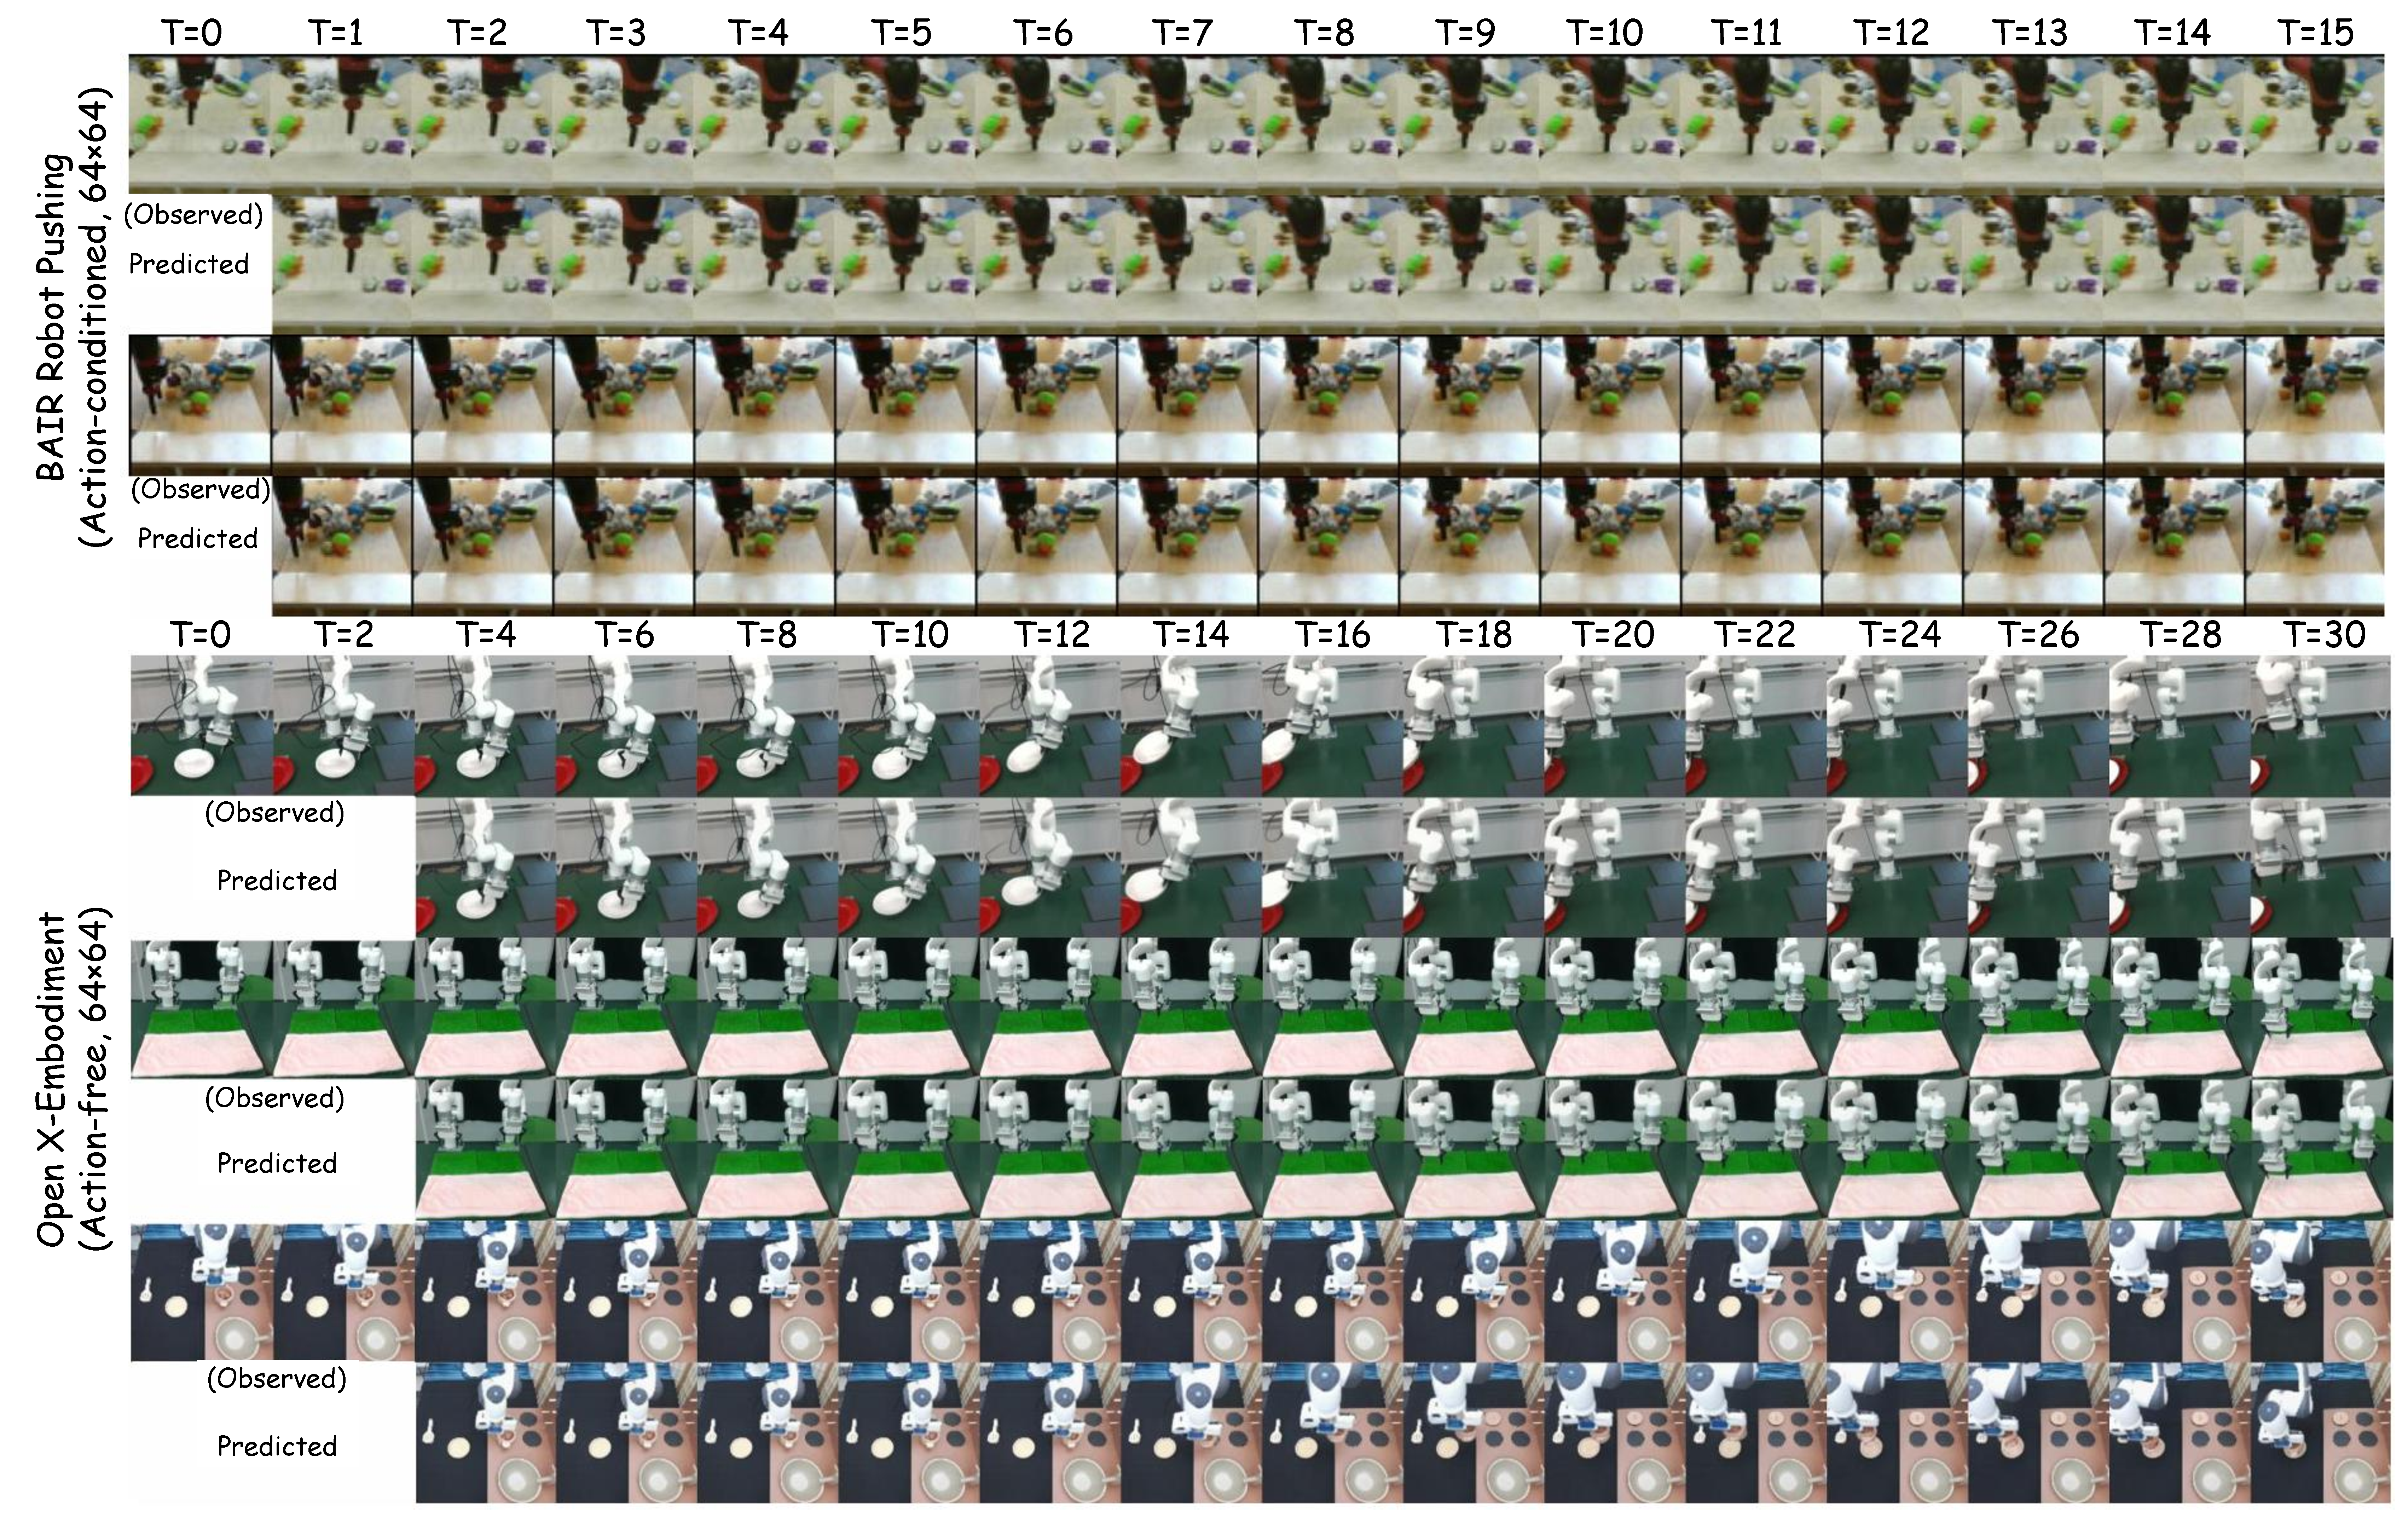
\includegraphics[width=1.0\linewidth]{fig_exp/fig64.pdf}
    \caption{\textbf{Visualization on BAIR and OpenX-Embodiment datasets.}}
    \label{fig_64}
    \vspace{-3ex}
\end{figure*}

\begin{figure*}[t]
    \centering
    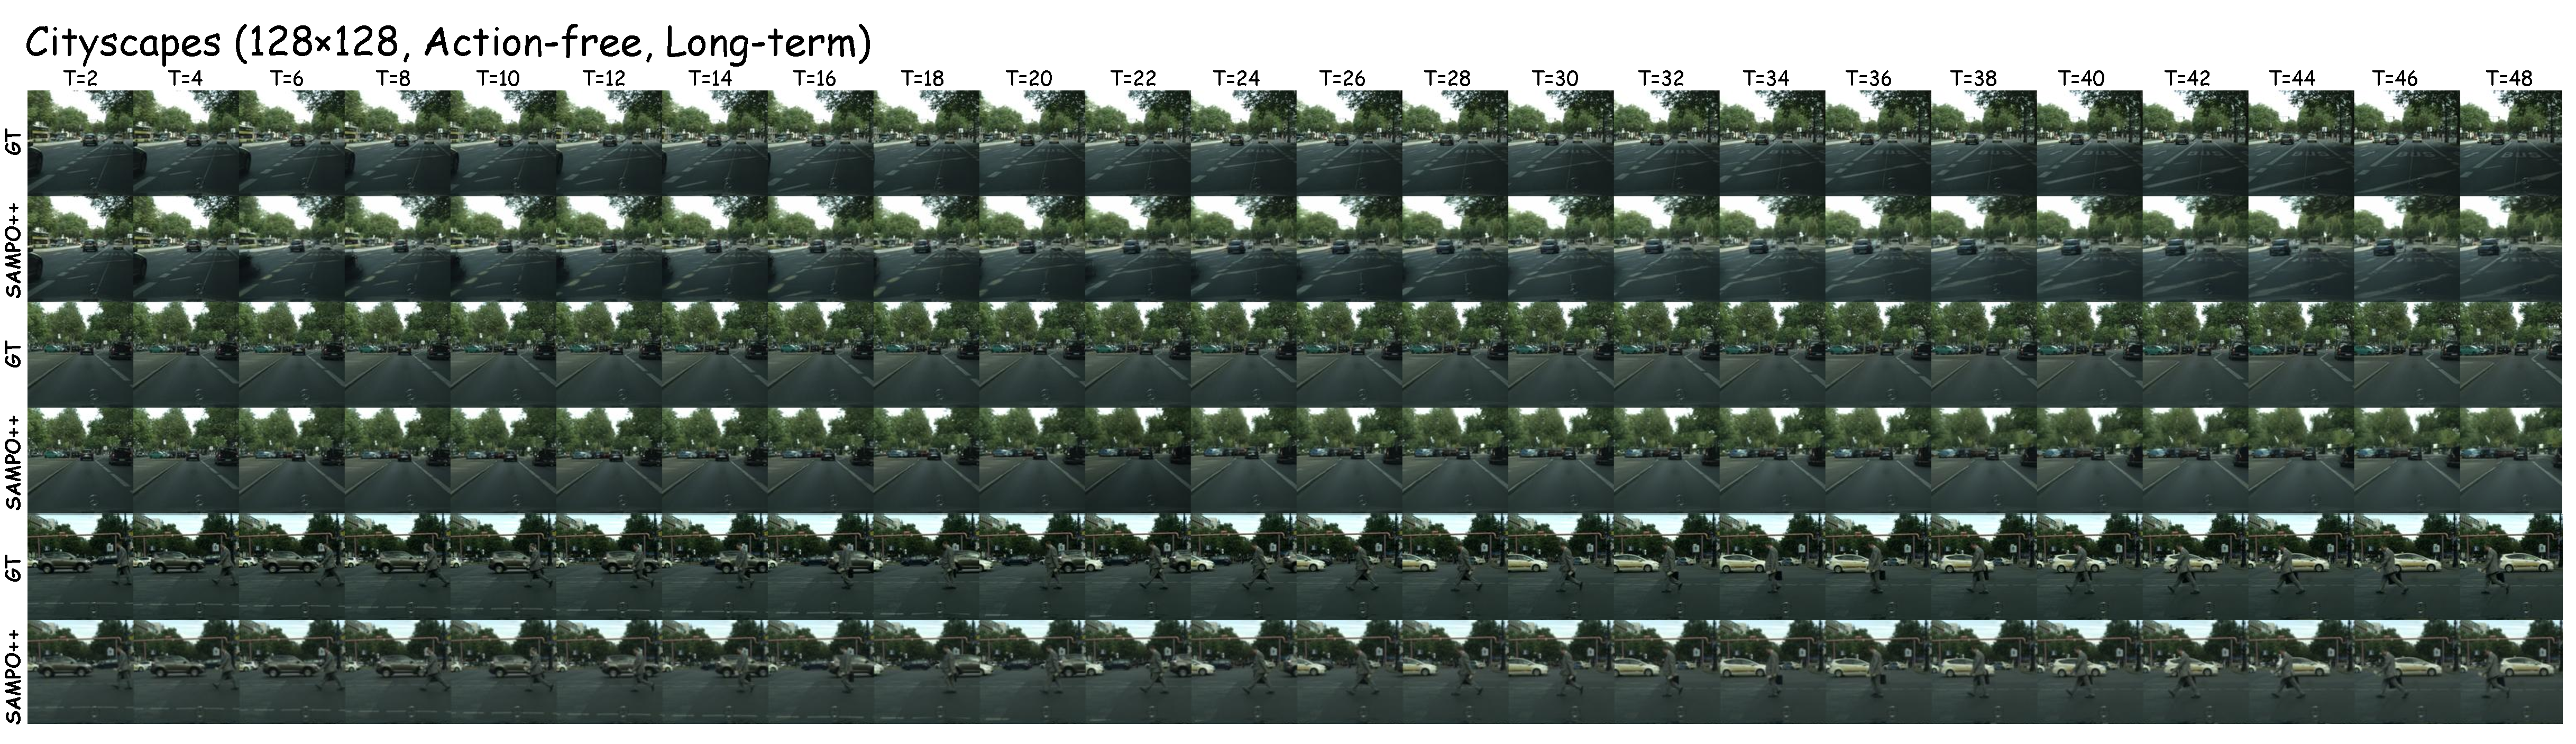
\includegraphics[width=1.0\linewidth]{fig_exp/fig_city.pdf}
    \caption{\textbf{Long-term video prediction on the Cityscapes dataset.} We visualize three distinct driving scenarios. Even over long-horizon generation, SAMPO++ excels at sustaining realistic scene dynamics and maintaining high spatiotemporal coherence without structural degradation. Zoom in for a better view.}
    \label{fig_city}
    \vspace{-3ex}
\end{figure*}

\begin{figure*}[t]
    \centering
    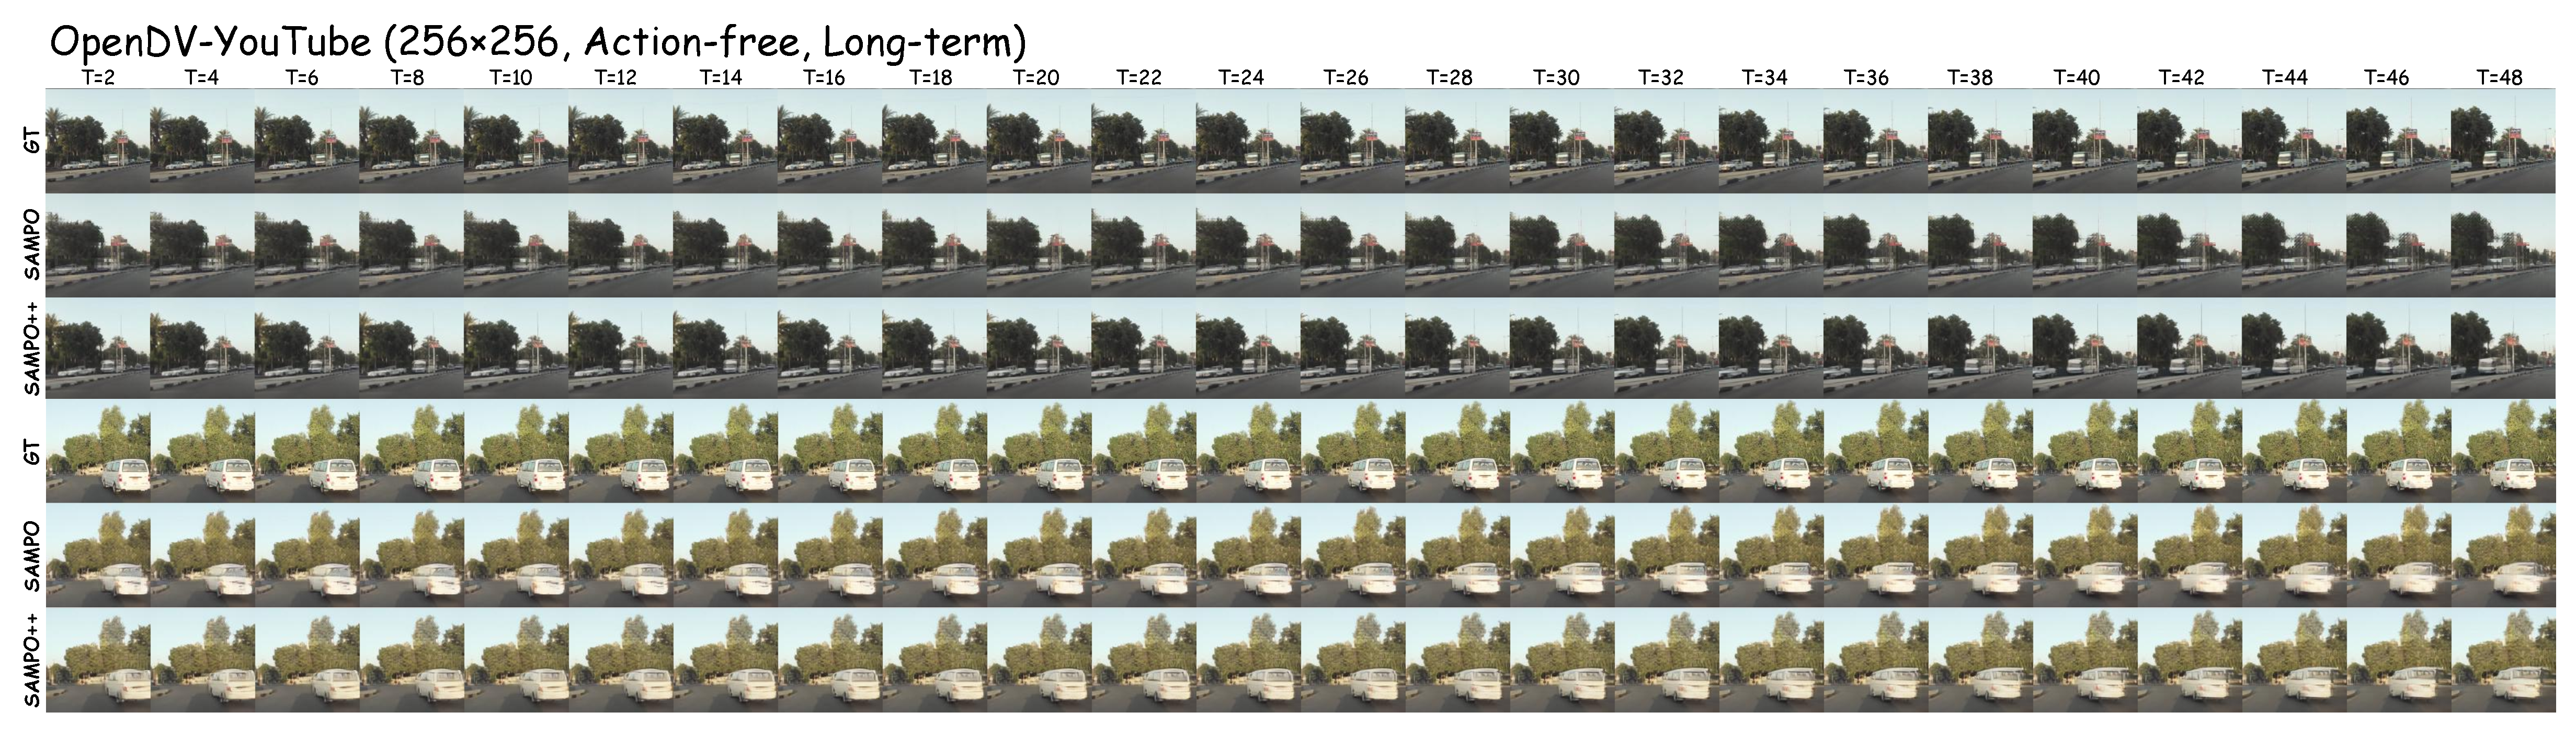
\includegraphics[width=1.0\linewidth]{fig_exp/figopendv.pdf}
    \caption{\textbf{High-resolution long-term video prediction on OpenDV-YouTube dataset.} We visualize highly complex, in-the-wild driving scenarios. While SAMPO suffers from severe temporal degradation in unconstrained driving scenarios, SAMPO++ effectively maintains robust dynamic modeling and strongly resists visual artifacts.}
    \label{fig_opendv}
    \vspace{-4ex}
\end{figure*}

\begin{figure}[t]
    \centering
    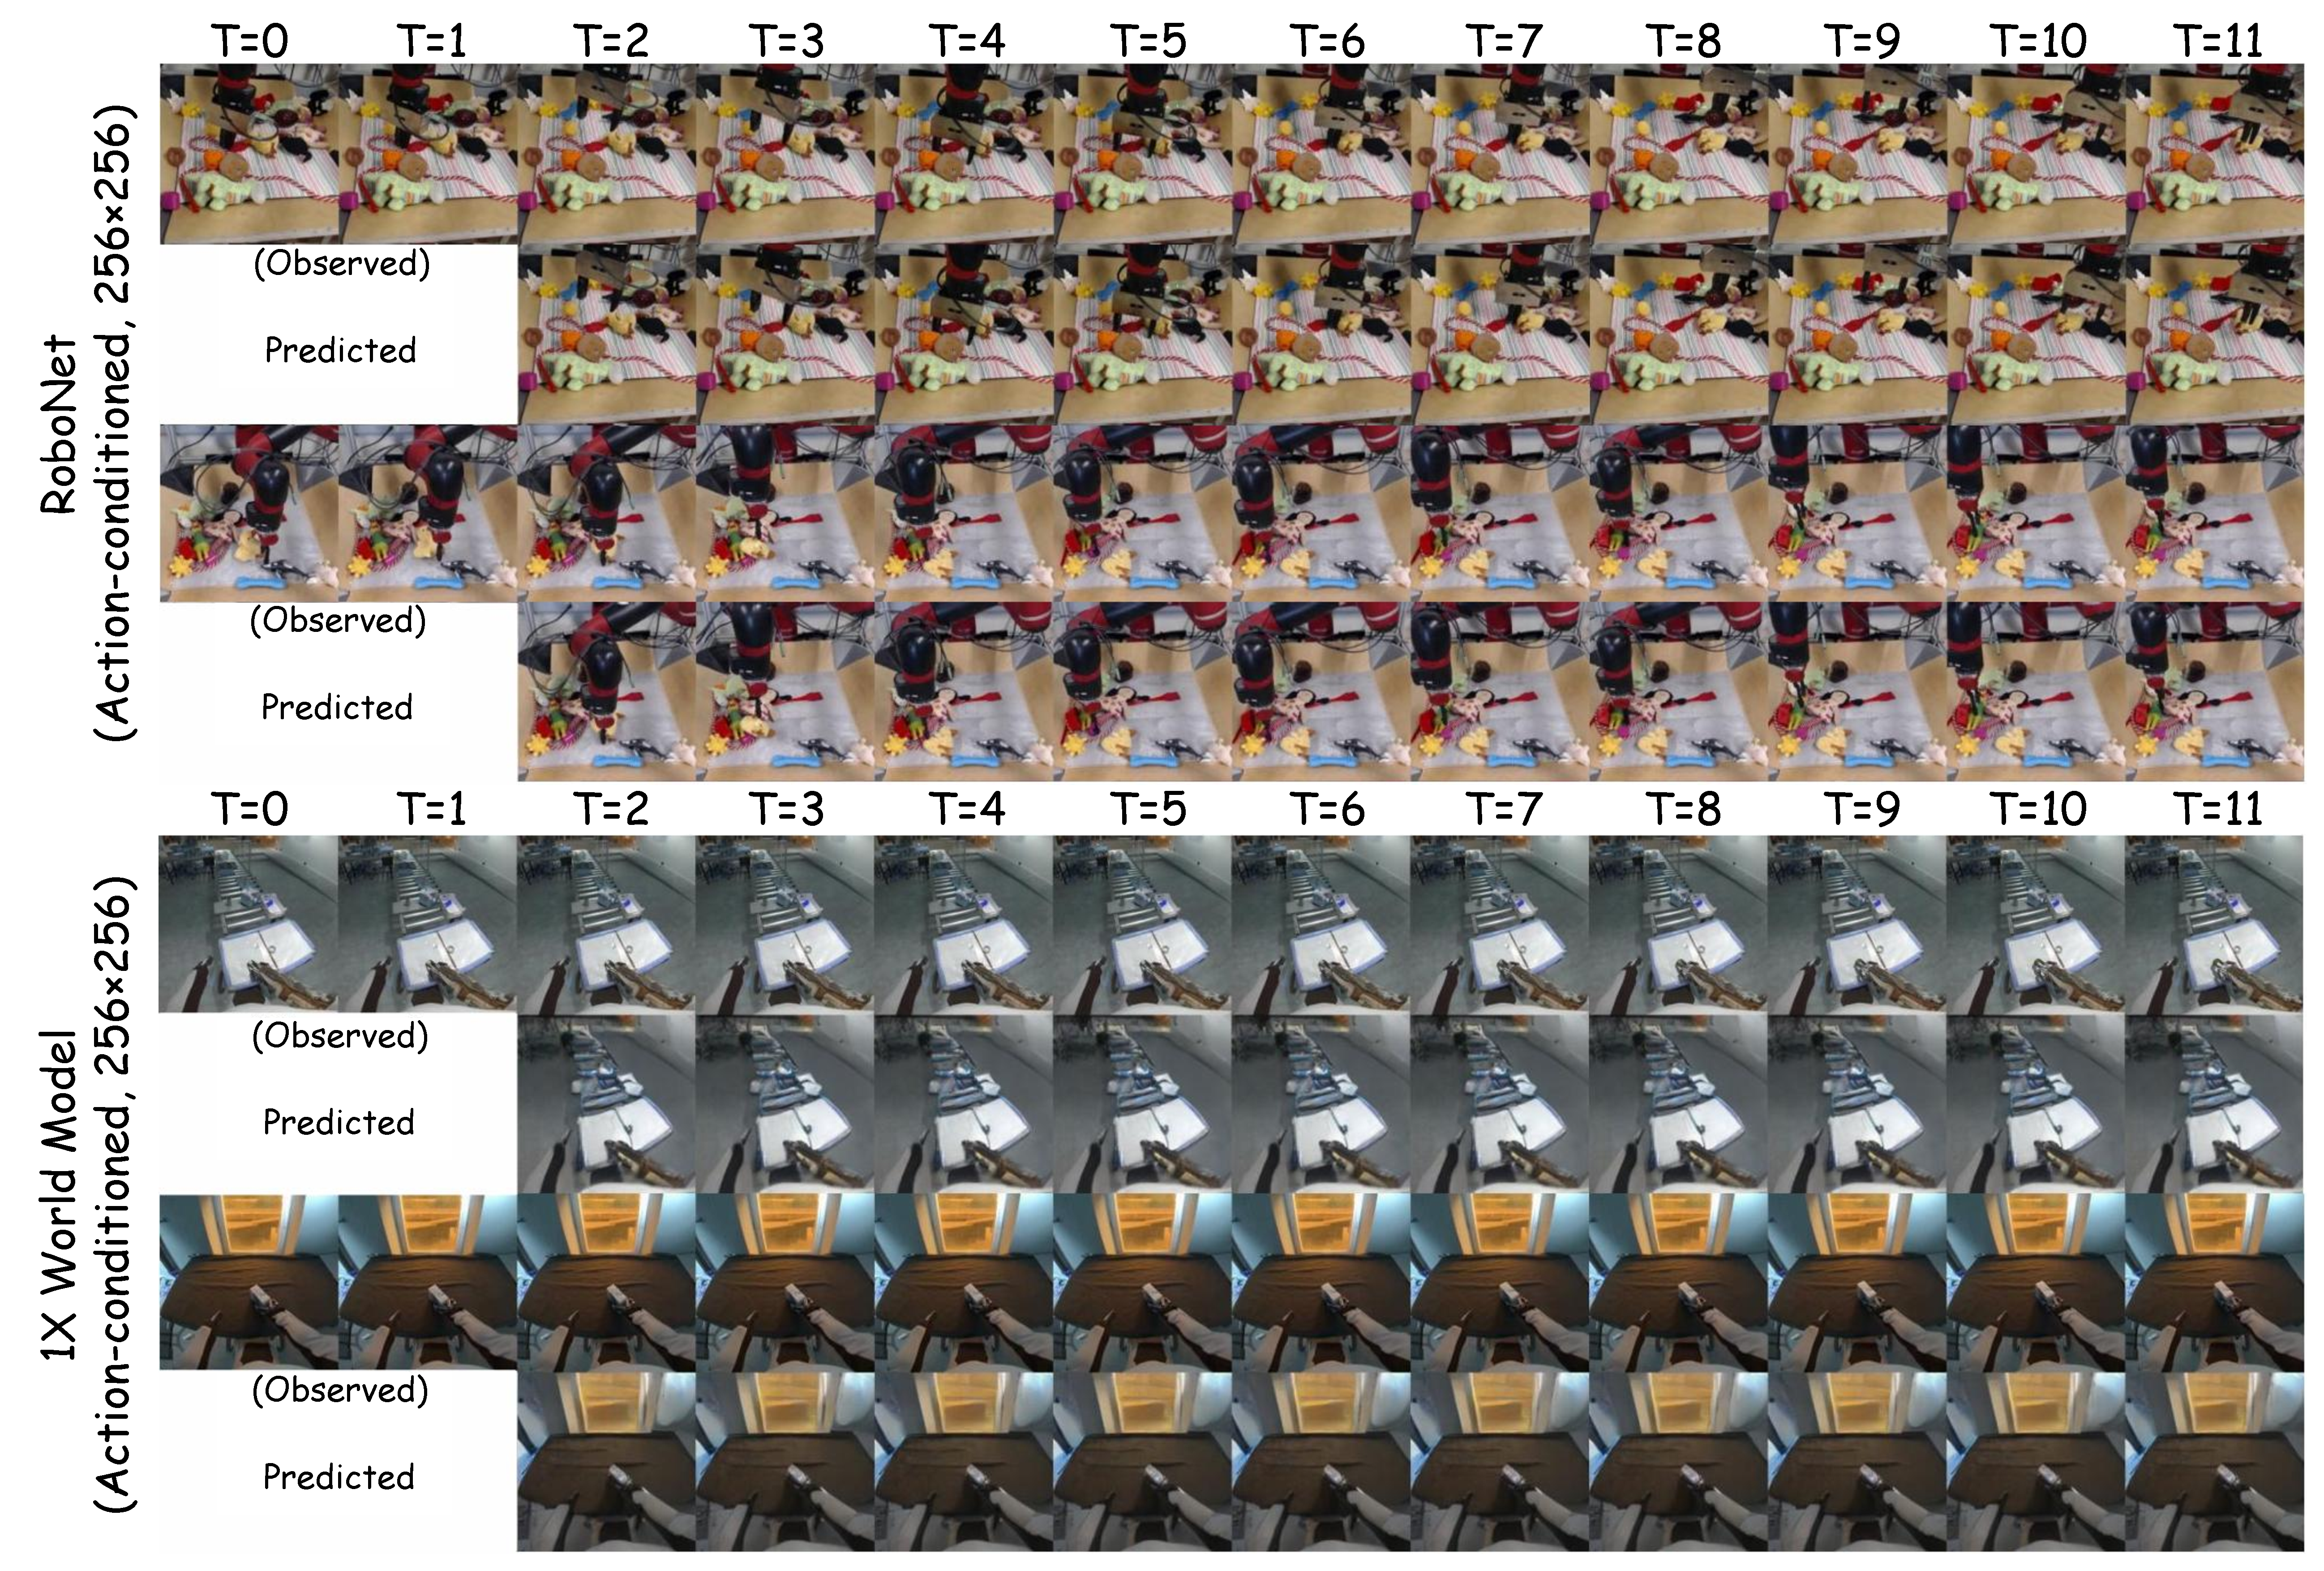
\includegraphics[width=1.0\linewidth]{fig_exp/fig256.pdf}
    \caption{\textbf{Visualization on RoboNet and 1X World Model.}}
    \label{fig_256}
    \vspace{-3ex}
\end{figure}

\begin{figure}[t]
    \centering
    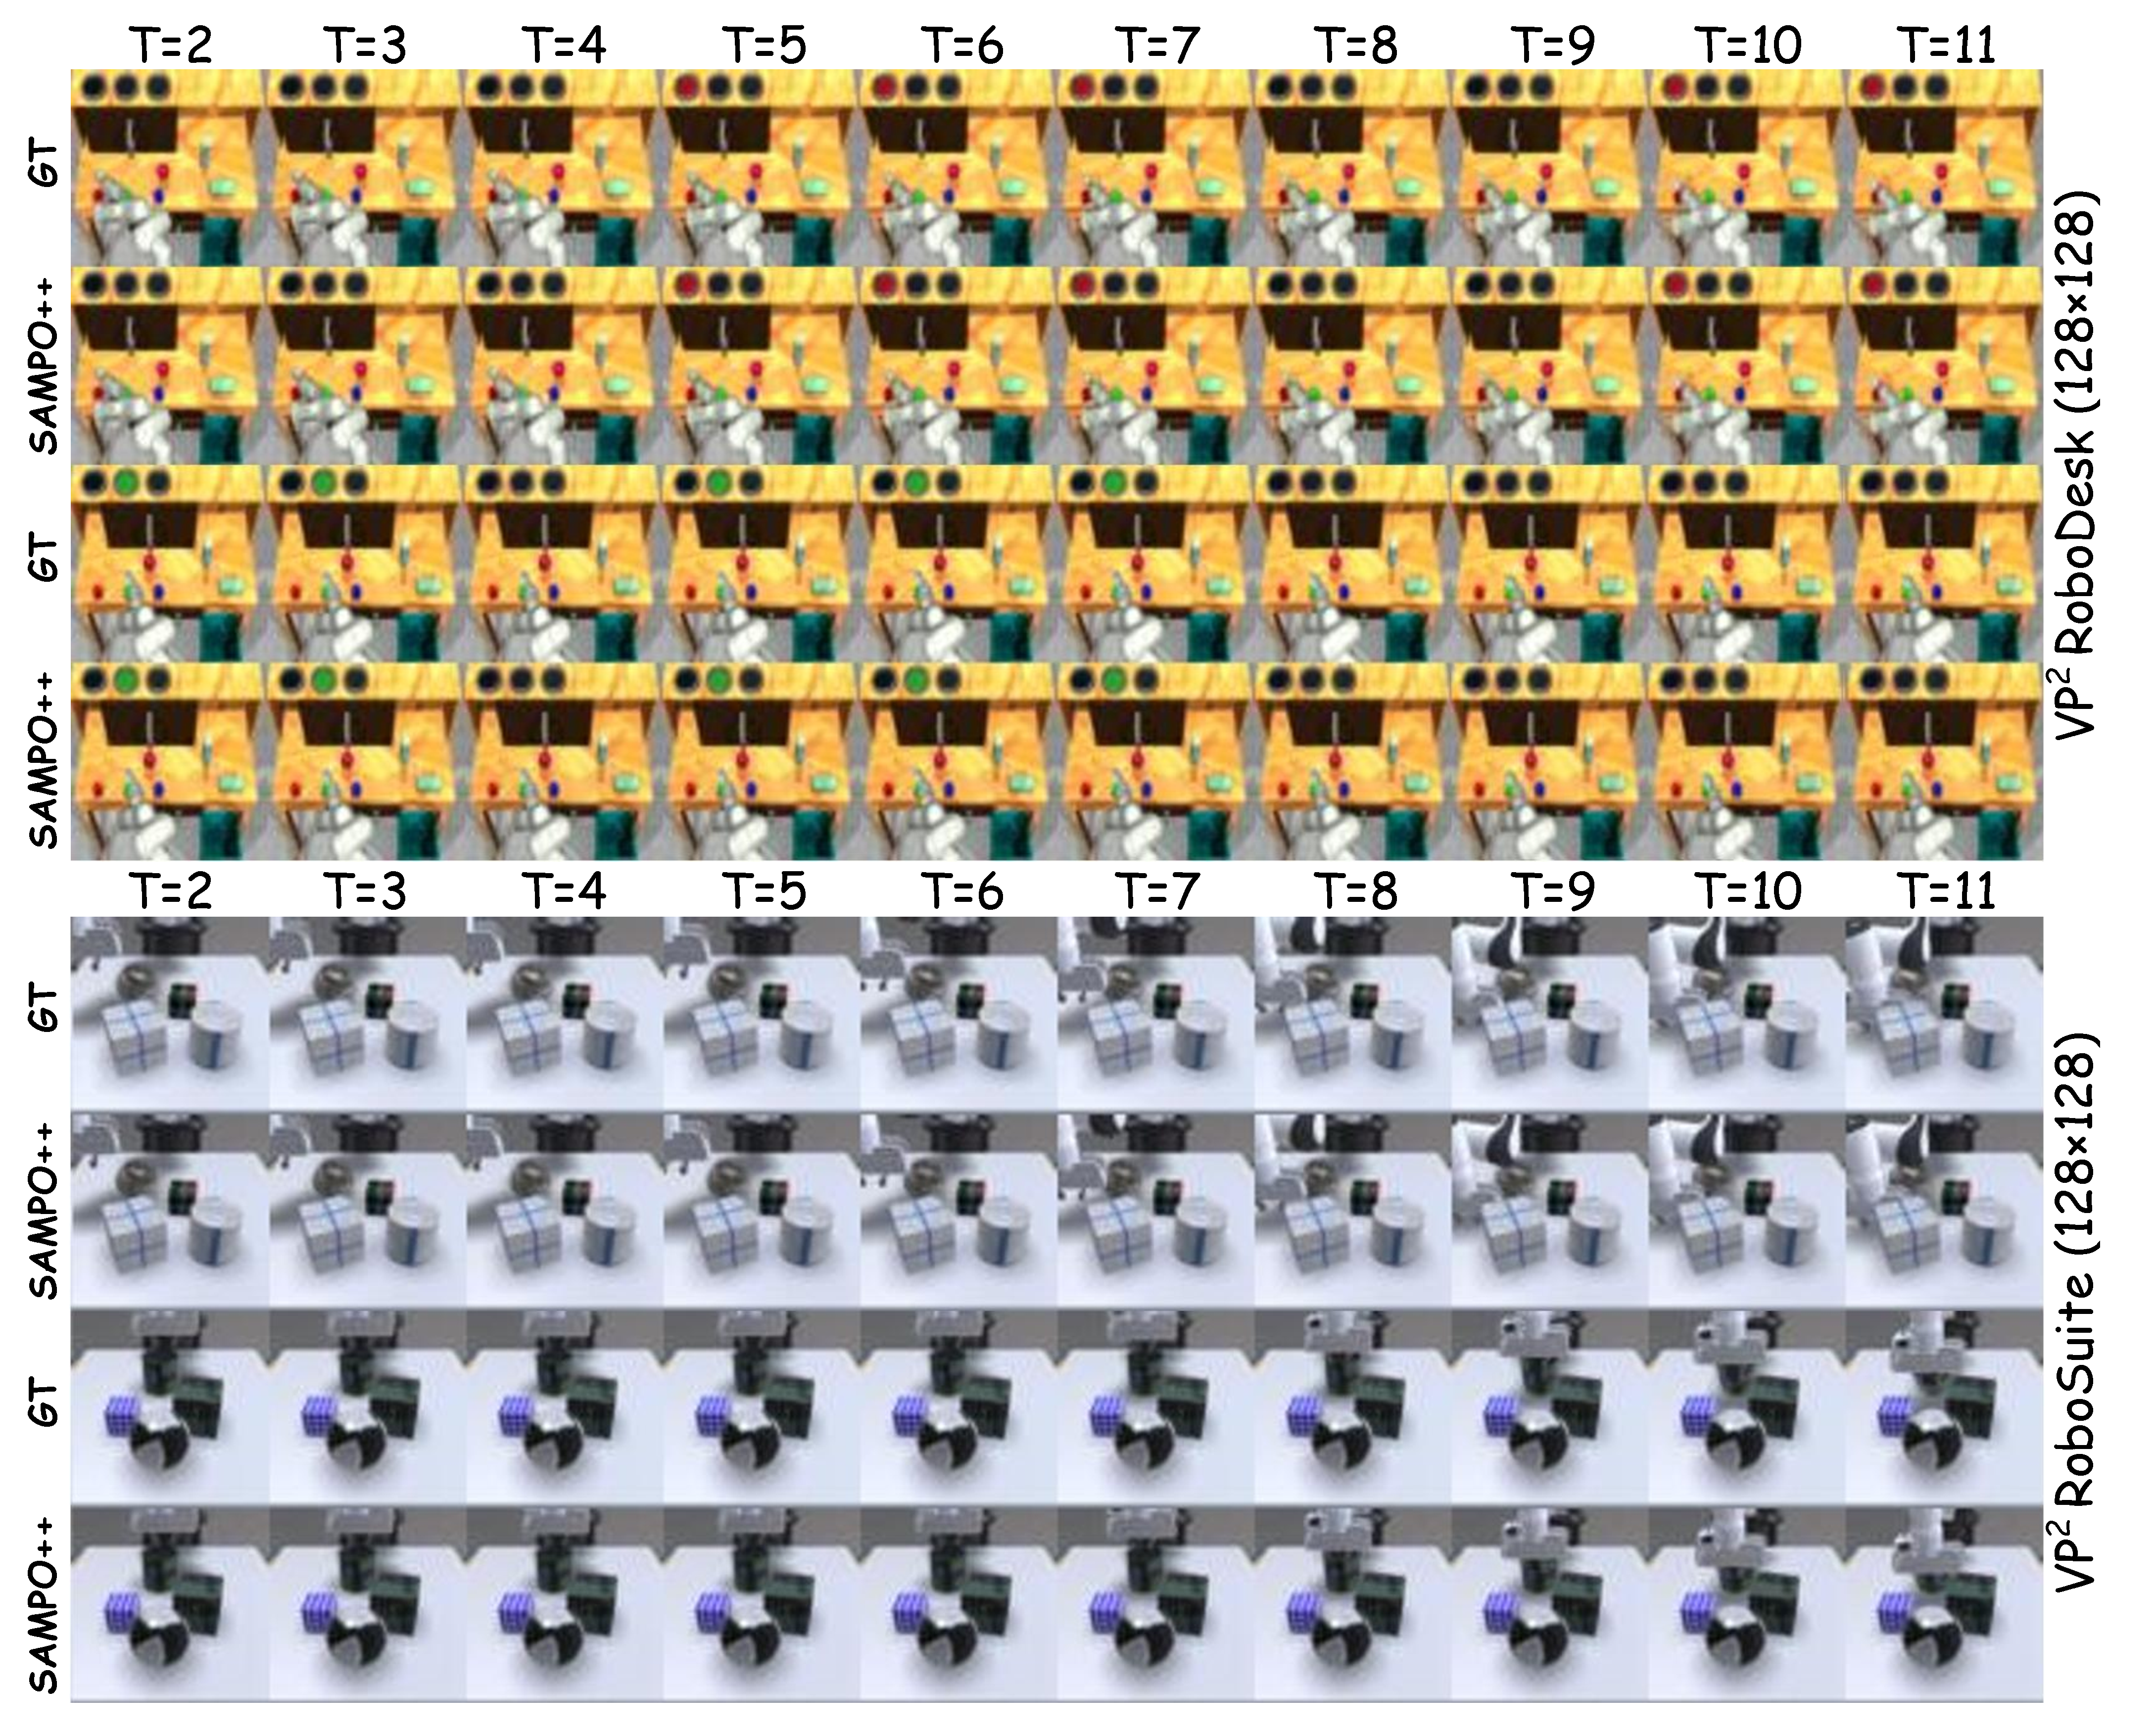
\includegraphics[width=1.0\linewidth]{fig_exp/fig_exp_vp2.pdf}
    \caption{\textbf{Visualization on the VP$^2$ benchmark.} We visualize two manipulation tasks from both the RoboDesk and RoboSuite environments.}
    % For each task, odd rows display the ground-truth observations, while even rows show the future trajectories predicted by SAMPO++.
    \label{fig_exp_vp2}
    \vspace{-3ex}
\end{figure}

\begin{figure}[t]
    \centering
    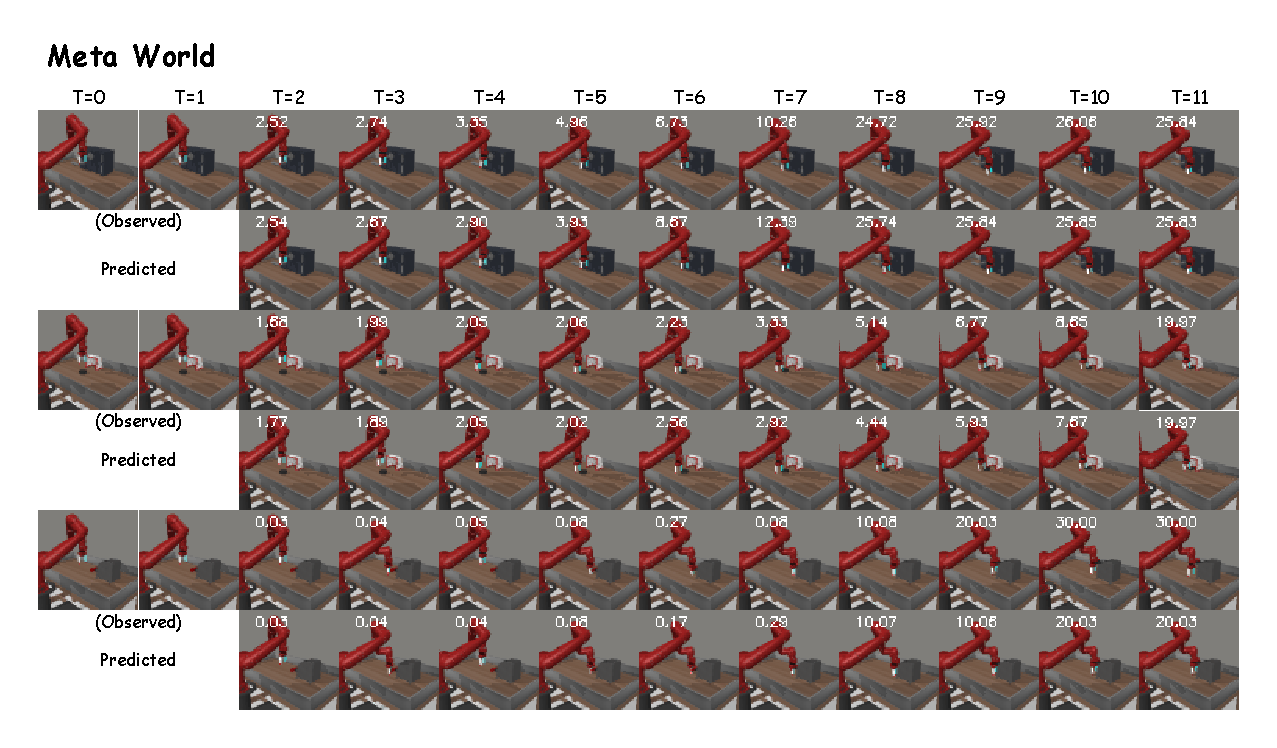
\includegraphics[width=1.0\linewidth]{fig_exp/fig_MW.pdf}
    \caption{\textbf{Visualization on the Meta-World tasks.} Each row corresponds to a different task: \textit{Coffee Push}, \textit{Door Lock}, \textit{Handle Pull Side}. Both actual reward and predicted reward are shown in the upper left corner.}
    \label{fig_MW}
    \vspace{-2ex}
\end{figure}

\subsection{Qualitative Analysis \& Visualization}

To contextualize our quantitative findings, we present a comprehensive qualitative analysis of SAMPO++ across diverse domains. Through a comparative visual assessment against ground-truth observations, we demonstrate the model's visual fidelity, physical plausibility, and strict adherence to action conditioning.

\textbf{Robotic Manipulation across Resolutions.} Figure~\ref{fig_64} showcases sampled rollouts on the BAIR and Open X-Embodiment datasets, illustrating the model's capacity to maintain spatiotemporal coherence across highly diverse manipulation trajectories at standard resolutions. Extending this to high-resolution generation, Figure~\ref{fig_256} presents $256 \times 256$ rollouts on the RoboNet and 1X World Model datasets. Here, SAMPO++ accurately synthesizes fine-grained physical details—such as subtle humanoid articulations—while preserving object permanence over extended horizons.

\textbf{Action-Conditioned Rollouts for Control.} Moving beyond passive video prediction, we examine interactive rollouts conditioned on specific action sequences. Figure~\ref{fig_exp_vp2} illustrates representative tasks from the $\text{VP}^2$ benchmark. By contrasting the predicted trajectories with ground-truth observations, we verify that the generated dynamics strictly obey the injected control signals and accurately simulate continuous physical interactions. Furthermore, Figure~\ref{fig_MW} demonstrates long-term rollouts on Meta-World manipulation tasks. The model reliably predicts both the visual observations and the corresponding task rewards at each step, yielding a robust neural simulator for downstream planning and policy learning.

\textbf{In-the-Wild and Autonomous Driving Generalization.} Finally, we demonstrate the scalability of our continuous-flow framework to complex, unconstrained environments. Figure~\ref{fig_city} displays long-term video prediction on the Cityscapes dataset, where SAMPO++ successfully renders dynamic traffic scenarios and preserves background structural integrity despite rapid viewpoint transformations. To further push these boundaries, Figure~\ref{fig_opendv} visualizes high-resolution ($256 \times 256$) long-horizon rollouts on uncurated internet videos from the OpenDV-YouTube dataset. Even when confronted with massive pixel displacements and unpredictable ego-motion, the model maintains robust spatiotemporal coherence, confirming its strong generalization capabilities in real-world driving scenarios.
